%-------------------------------------------------------------------------------------
%	PACKAGES AND THEMES
%-------------------------------------------------------------------------------------
\documentclass{beamer}
\setbeamercovered{transparent}
\setbeamercolor{local structure}{fg=black}
\setbeamertemplate{caption}{\raggedright\insertcaption\par}
\usefonttheme[onlymath]{serif}

\mode<presentation> {
	
	% The Beamer class comes with a number of default slide themes
	% which change the colors and layouts of slides. Below this is a list
	% of all the themes, uncomment each in turn to see what they look like.
	
	%\usetheme{default}
	%\usetheme{AnnArbor}
	%\usetheme{Antibes}
	%\usetheme{Bergen}
	%\usetheme{Berkeley}
	%\usetheme{Berlin}
	%\usetheme{Boadilla}
	\usetheme{CambridgeUS}
	%\usetheme{Copenhagen}
	%\usetheme{Darmstadt}
	%\usetheme{Dresden}
	%\usetheme{Frankfurt}
	%\usetheme{Goettingen}
	%\usetheme{Hannover}
	%\usetheme{Ilmenau}
	%\usetheme{JuanLesPins}
	%\usetheme{Luebeck}
	%\usetheme{Madrid}
	%\usetheme{Malmoe}
	%\usetheme{Marburg}
	%\usetheme{Montpellier}
	%\usetheme{PaloAlto}
	%\usetheme{Pittsburgh}
	%\usetheme{Rochester}
	%\usetheme{Singapore}
	%\usetheme{Szeged}
	%\usetheme{Warsaw}
	
	% As well as themes, the Beamer class has a number of color themes
	% for any slide theme. Uncomment each of these in turn to see how it
	% changes the colors of your current slide theme.
	
	%\usecolortheme{albatross}
	%\usecolortheme{beaver}
	%\usecolortheme{beetle}
	%\usecolortheme{crane}
	%\usecolortheme{dolphin}
	%\usecolortheme{dove}
	%\usecolortheme{fly}
	%\usecolortheme{lily}
	\usecolortheme{orchid}
	%\usecolortheme{rose}
	%\usecolortheme{seagull}
	%\usecolortheme{seahorse}
	%\usecolortheme{whale}
	%\usecolortheme{wolverine}
	
	%\setbeamertemplate{footline} % To remove the footer line in all slides uncomment this line
	%\setbeamertemplate{footline}[page number] % To replace the footer line in all slides with a simple slide count uncomment this line
	
	%\setbeamertemplate{navigation symbols}{} % To remove the navigation symbols from the bottom of all slides uncomment this line
}

\usepackage{graphicx} % Allows including images
\usepackage{booktabs} % Allows the use of \toprule, \midrule and \bottomrule in tables
\usepackage{caption}
\captionsetup{font=scriptsize,labelfont=scriptsize}
\usepackage{amssymb}
\usepackage{bm}
%\usepackage{enumitem}
\usepackage{amsfonts}
\usepackage[colorinlistoftodos,prependcaption,textsize=small]{todonotes}
%-------------------------------------------------------------------------------------
%	TITLE PAGE
%-------------------------------------------------------------------------------------

\title[Large-Scale Data Analysis Techniques]{A Review on Multi-Label Learning Algorithms} % The short title appears at the bottom of every slide, the full title is only on the title page

\author[Sissy Themeli, Nikiforos Pittaras]{Min-Ling Zhang and Zhi-Hua Zhou} % Your name
\institute[DI-UOA] % Your institution as it will appear on the bottom of every slide, may be shorthand to save space
{
	IEEE Transactions On Knowledge And Data Engineering\\ % Your institution for the title page
	\medskip
}
\date{\today} % Date, can be changed to a custom date

\begin{document}
	
	\begin{frame}
	\titlepage % Print the title page as the first slide
\end{frame}

\begin{frame}
\frametitle{Overview} % Table of contents slide, comment this block out to remove it
\tableofcontents % Throughout your presentation, if you choose to use \section{} and \subsection{} commands, these will automatically be printed on this slide as an overview of your presentation
%\setbeamercolor{section in toc}{fg=black}
%\setbeamercolor{subsection in toc}{fg=black}
\end{frame}

%-------------------------------------------------------------------------------------
%	PRESENTATION SLIDES
%-------------------------------------------------------------------------------------

\section{Introduction} % Sections can be created in order to organize your presentation into discrete blocks, all sections and subsections are automatically printed in the table of contents as an overview of the talk
\subsection{Multi-label learning}
%------------------------------------------------
\begin{frame}
\Huge{\centerline{Introduction}}
\end{frame}
%------------------------------------------------
\begin{frame}
\frametitle{\insertsection : \insertsubsection}
\onslide<2-> {Learning $\rightarrow$ build a model from data, to accomplish a task}
\begin{itemize}
  	\item <3-> Supervised: we have both data \emph{and labels}
	\item <4-> Applied to classification in this study
\end{itemize}
\onslide <5-> {Supervised classification:}
\begin{itemize}
\item[$\bullet$] <6-> Given input data $X$ and labels  $Y$,
  learn the function $f: X \rightarrow Y$ 
\item[$\bullet$] <7-> $f(x_i, y_i) = r$ where $r\in \mathbb{R}$ is the confidence that $y_i$ characterizes $x_i$
\item[$\bullet$] <8-> Assume that $x_i$ belongs to $y_i$ if $r \ge $ $t(x_i)$
\begin{itemize}%[label={$\checkmark$}]
\item[$\checkmark$] <9-> $t(\cdot)$ can be a predetermined constant function or learned from $X$
\end{itemize}
\end{itemize}

\onslide <10-> {Single-label learning}
\begin{itemize}
\item[$\bullet$] <11-> Dataset $\{ (x_i, y_i)\}, i = 1, \dots N, x \in X, y \in Y=\{y_1,\dots,y_q\}$
\end{itemize}

\onslide <12->{Multi-label learning}
\begin{itemize}
\item[$\bullet$] <13-> Multi-label dataset: Multiple labels per instance. $\{ (x_i, \bm{y}_i)\}, i = 1, \dots N, x \in X, \bm{y} \in \mathbb{P}(Y)$
% \item Learn a model $f: X \times Y \rightarrow r$

\end{itemize}
\end{frame}
%------------------------------------------------
%------------------------------------------------
\subsection{Algorithm Strategies}
\begin{frame}
\frametitle{\insertsection : \insertsubsection}
\onslide <2->{Label search space $\mathbb{S_Y}$ grows exponentially as a function of $|Y|=q$}
\begin{itemize}
\item[$\triangleright$] <3-> e.g. for $q=20, |\mathbb{S_Y}| = 2 ^ {|\mathbb{P(Y)}|} = 2^{20} \ge 10^6$
\end{itemize}
\onslide <4->{Solution: integrate in the learning process potential label correlations.

In this work the authors group M-L algorithms in three categories:}

\begin{enumerate}
\item <5->First-order strategies
\begin{itemize}
\item[$\circ$] <6-> Ignore label correlations
\item[$\circ$] <7-> Often transform M-L problem to multiple, single-label problems
  and combine the per-label results
\item[$\circ$] <8-> Simple, scalable, suboptimal
\end{itemize}
\item <9-> Second-order strategies
\begin{itemize}
\item[$\circ$] <10-> Consider \emph{pairwise} label relations
\item[$\circ$] <11-> Good trade-off between generalization performance and scalability
\item[$\circ$] <12-> Lacking in some real-world applications
\end{itemize}
\item <13->Higher-order strategies
\begin{itemize}
\item[$\circ$] <14-> Capture more complicated label interdependencies
\item[$\circ$] <15-> Strong modeling capabilities that can capture complex relationships
\item[$\circ$] <16-> Computationally demanding, less scalable
\end{itemize}

\end{enumerate}
\end{frame}

%------------------------------------------------
\subsection{Evaluation Metrics}
\begin{frame}
\frametitle{\insertsection : \insertsubsection}
\onslide <2->{Extension of single-label metrics to the M-L case.

Grouped into two categories and perspectives:}
\begin{itemize}
\item[$\bullet$] <3-> \emph{Example-based: }Evaluates multi-labeled performance on each example, extrapolate to whole dataset
\begin{itemize}
\item[$\circ$] <4-> \emph{Classification perspective:}
\begin{itemize}
\item[$-$] <5-> Subset Accuracy, Hamming Loss
\item[$-$] <6-> Precision, Recall,  F$^\beta$ -measure
\end{itemize}
\item[$\circ$] <7-> \emph{Ranking perspective:} one-error, coverage, ranking loss, average precision
\end{itemize}
\item[$\bullet$] <8-> \emph{Label-based: }Evaluates performance on each label separately, extrapolate to whole label set
\begin{itemize}
\item[$\circ$] <9-> Classification perspective: Macro/Micro averaging techniques for single-label example-based, classification-perspective measures
\item[$\circ$] <10-> Ranking perspective: Macro/Micro averaging for AUC
\end{itemize}
\end{itemize}
\onslide <11->{$\ast$ Ideally, classifiers should be trained to optimize \emph{multiple} metrics}
\end{frame}
%------------------------------------------------
\section{Multi-label Learning Algorithms}
%------------------------------------------------
\subsection{Categorization}
%------------------------------------------------
\begin{frame}
\Huge{\centerline{Multi-label Learning Algorithms}}
\end{frame}
%------------------------------------------------
\begin{frame}
\frametitle{\insertsection : \insertsubsection}

\onslide <2->{Group algorithms in two categories:}
\begin{itemize}
\item[$\bullet$] <3-> \emph{Problem Transformation Methods:}

\begin{itemize}
\item[$\circ$] <4-> Transform the learning problem into other, managable (often
  single-label) learning
  problems 
\item[$\circ$] <5-> ``Fit data to algorithm'' philosophy
\end{itemize}

\item[$\bullet$] <6-> \emph{Algorithm Adaptation Methods:}
\begin{itemize}
\item[$\circ$] <7-> Adapt popular learning techniques to deal with multi-label data directly
\item[$\circ$] <8-> ``Fit algorithm to data'' philosophy
\end{itemize}
\end{itemize}

\onslide <9->{Authors include algorithms that:}
\begin{itemize}
\item[$\checkmark$] <10-> Has broad, noteworthy or unique characteristics
\item[$\checkmark$] <11-> Has important impact, leading to a number follow-up related methods
\item[$\checkmark$] <12-> Is influential and highly-cited in multi-label learning
\end{itemize}
\end{frame}
%------------------------------------------------
\subsection{Problem Transformation Methods}
%------------------------------------------------
\begin{frame}
\Huge{\centerline{Problem Transformation Methods}}
\end{frame}
%------------------------------------------------
\begin{frame}
\frametitle{\insertsection : \insertsubsection}
\begin{figure}
\begin{center}
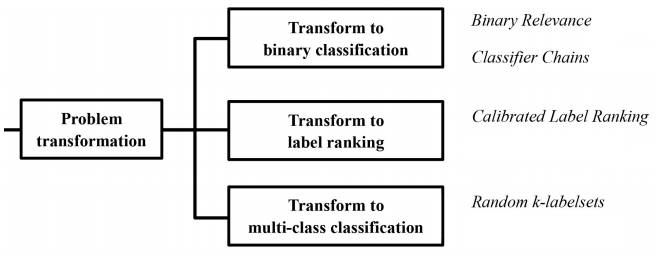
\includegraphics[scale = 0.7]{images/pt.png}
\end{center}
\end{figure}
\end{frame}
%------------------------------------------------
\begin{frame}
\frametitle{Binary Relevance}

\begin{itemize}
\item[$\bullet$] <2-> Decompose multi-label problem to $|Y|=q$ independent binary classification problems
\item[$\bullet$] <3-> Construct $q$ binary (one-vs-all) training sets (one for each $y_i$)
\item[$\bullet$] <4-> Independently train each classifier $h_i(x)$ on its respective dataset

\item[$\bullet$] <5-> Predict labels of an unseen $x$ by evaluating each classifier $h_i(x)$
\item[$\bullet$] <6-> Assign label $y_i$ according to $r = h_i(x)$ and the
  thresholding setting 
\end{itemize}

\onslide <7->{Pros \& cons:}
\begin{itemize}
\item[$\bullet$] <8-> Simple, one-vs-rest scheme $\rightarrow$ easily parallelizable
\item[$\bullet$] <9-> Sensitive to class-imbalanced data\footnote{Very different
    number of pos. and neg. examples for a class}
\item[$\bullet$] <10-> Ignores label correlations (first-order method)
\end{itemize}

\end{frame}
%------------------------------------------------

\begin{frame}
\frametitle{Classifier chains}
\begin{itemize}
\item[$\bullet$] <2-> Reorder the label $Y$ set using a permutation function $f_p$ 
\item[$\bullet$] <3-> Transform into a \emph{chain} of binary classification problems
\item[$\bullet$] <4-> Enrich representations at step $j$ by concatenating each $x_i$ with the confidence of preceeding $1,\dots,j-1$-th classifiers
\item[$\bullet$] <5-> Predict relevant labels for unknown instances by iteratively traversing the classifier chain
\end{itemize}

\onslide <6->{Pros \& cons:}
\begin{itemize}
\item[$\bullet$] <7-> High-order method: exploitation of label correlations to a degree, but in a random manner
\item[$\bullet$] <8-> Highly sensitive to $f_p$. Running multiple chain executions in an ensemble attempt to overcome this dependency.
\item[$\bullet$] <9-> Iterative operation prevents parallel implementation
\end{itemize}
\end{frame}
%------------------------------------------------

\begin{frame}
\frametitle{Calibrated Label Ranking}
\begin{itemize}
\item[$\bullet$] <2-> Transform into a label pairwise comparison ranking problem
\item[$\bullet$] <3-> For $q$ labels, generate $q(q-1)/2$ binary classifiers by pairwise comparison and use a binary algorithm $h_{jk}(x)$
\item[$\bullet$] <4-> Construct training sets $D_{jk} : \{x_i, Y_i | y_j \in Y_i \oplus y_k \in Y_i\}$. System votes for each example and if $h_{jk}(x) >0$,$x_i$ is associated with $y_j$, otherwise with $y_k$
\item[$\bullet$] <5-> For an unknown instance, all classifiers' votes are aggregated
  and resulting labels are ranked according to the total confidence $r$
\item[$\bullet$] <6-> A virtual label $y_v$ is learned as a threshold, serving as the artificial splitting point between relevant and irrelevant labels
\end{itemize}
\onslide <7->{Pros \& cons:}
\begin{itemize}
\item[$\bullet$] <8-> Second-order approach algorithm. One-vs-one scheme.
\item[$\bullet$] <9-> Pairwise comparison smooths out the class-imbalance problem
\item[$\bullet$] <10-> Number of classifiers is quadratic to $|Y|$ (compared to linear for BR)
\begin{itemize}
\item[$\circ$] <11-> Pruning methods to reduce the search space
\end{itemize}
\end{itemize}
\end{frame}
%------------------------------------------------
\begin{frame}
\frametitle{Random k-Labelsets}
\begin{itemize}
\item[$\bullet$] <2-> Decompose to an ensemble of multi-class classification problems
\item[$\bullet$] <3-> Each component targets a random subset of $\mathbb{P}(Y)$ (that
  also appears in $X$), classified with Label Powerset (LP) techniques:
\begin{itemize}
\item[$\circ$] <4-> Transform to single-label data by treating each distinct labelset
  as a new class $\rightarrow$ multi to single label problem
\item[$\circ$] <5-> Each example is reassigned with the new mapped class and classified through regular single-label classification
\item[$\circ$] <6-> M-L classify $x$ with $y_i$ when the votes received for $y_i$ from the ensemble exceed half the max possible it can get
\end{itemize}
\end{itemize}
\onslide <7->{Pros \& cons:}
\begin{itemize}
\item[$\bullet$] <8-> High-order approach algorithm
\item[$\bullet$] <9-> Data-sensitive: Cannot generalize to labelsets not in the training set, too few examples for some labelsets
\item[$\bullet$] <10-> Large $Y$ implies high training complexity.
\item[$\bullet$] <11-> Improve by invoking an ensemble on random k-sized labelsets
\end{itemize}
\end{frame}
%------------------------------------------------
\subsection{Alogrithm Adaptation Methods}
%------------------------------------------------
\begin{frame}
\Huge{\centerline{Algorithm Adaptation Methods}}
\end{frame}
%------------------------------------------------
\begin{frame}
\frametitle{\insertsection : \insertsubsection}
\begin{figure}
\begin{center}
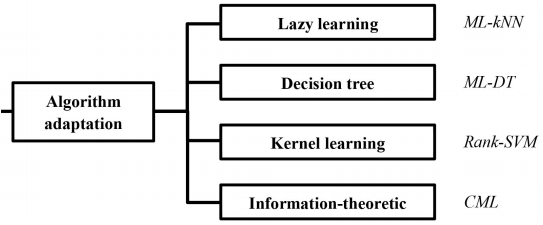
\includegraphics[scale = 0.75]{images/aa.png}
\end{center}
\end{figure}
\end{frame}
%------------------------------------------------
\begin{frame}
\frametitle{Multi-Label k-Nearest Neighbour}
\begin{itemize}
	\item[$\bullet$] <2-> Consider events $H_j \equiv (y_j \in Y_i)$, $C_j \equiv (\sum_{x_k \in N(x_i)} [\delta(y_j \in Y_k)])$
\item[$\bullet$] <3-> Compares the MAP probabilities: $P(K|C_j), K \in \{H_j, \neg H_j\}$ to decide if to include $y_j$ in the prediction. Compute with the Bayes' theorem.
\item[$\bullet$] <4-> Single-label priors $P(K)$ computed by smoothed frequency counting in the training data
\item[$\bullet$] <5-> Likelihoods $P(C_j|K)$ are computed as a function of:
\begin{itemize}
\item[$\circ$] <6-> $\kappa_j(r)$, the number of examples labelled $y_j$ with $r$ neighbours labelled $y_j$
\item[$\circ$] <7-> $\overset{\sim}{\kappa_j}(r)$, the number of examples not labelled $y_j$ with $r$ neighbours labelled $y_j$
\end{itemize}
\end{itemize}

\onslide <8->{Pros \& cons:}
\begin{itemize}
\item[$\bullet$] <9-> First-order approach, Bayesian reasoning
\item[$\bullet$] <10-> Decision boundary can be modified on-line via new instances
\item[$\bullet$] <11-> M-L class imbalance can be overcome by calculating the priors
\item[$\bullet$] <12-> Extensions proposed for label correlation exploitations
\end{itemize}
\end{frame}
%------------------------------------------------
\begin{frame}
\frametitle{Multi-label Decision Tree}
\begin{itemize}
\item[$\bullet$] <2-> Multi-label entropy is used to build a decision tree recursively
\item[$\bullet$] <3-> Split node at the $l$-th feature of $x$ such that the information gain criterion is maximized. Node partitions data according to $x_l = \theta$:
 $T \rightarrow \{T^-,T^+\}$, where $ x_{il} \leq \theta, x_i \in T^-$ and $ x_{il} > \theta, x_i \in T^+$
\item[$\bullet$] <4-> Recurse on subtrees until a stopping criterion is met (e.g. child size)
\item[$\bullet$] <5-> Single-label entropy is computed by considering labelsets as new classes
\item[$\bullet$] <6-> Assumes independence among labels to ensure low computational cost
\item[$\bullet$] <7-> Unseen instances are assigned the label of the majority of members of the leaf they arrive
\end{itemize}
\onslide <8->{Pros \& cons:}
\begin{itemize}
\item[$\bullet$] <9-> First-order algorithm, highly efficient
\item[$\bullet$] <10-> Assumes label independence
\item[$\bullet$] <11-> Pruning and ensemble strategies proposed
\end{itemize}
\end{frame}
%------------------------------------------------
\begin{frame}
\frametitle{Ranking Support Vector Machine}
\begin{itemize}
	\item[$\bullet$] <2-> $q$ linear classifiers $h_i(x)$, optimized with the empirical ranking loss
	\item[$\bullet$] <3-> Combine classifiers to discriminate label \emph{pairs}. Label pair $(j, k)$ decision hyperplane is: $h_{jk} = g(h_j, h_k) = \left<w_j-w_k, x_i \right> + b_j - b_k=0$
\item[$\bullet$] <4-> Consider signed distance of $x_i$ from the boundary of every
  relevant-nonrelevant label pair $(y_j,y_k) \in Y_i \times \bar Y_i$.
  % The pair's decision hyperplane is: $h_j, h_k$: $\left<w_j-w_k, x_i \right> + b_j - b_k=0$
\item[$\bullet$] <5-> The M-L margin is the minimum distance of $x_i$ from every  $Y_i \times \bar Y_i$
\item[$\bullet$] <6-> SVM $\rightarrow$ minimize loss \emph{and} maximize margin.

\item[$\bullet$] <7-> Ranks labels according to the singed distance
\item[$\bullet$] <8-> Non-linearity achievable through feature mapping and the kernel trick
\end{itemize}
\onslide <9->{Pros \& cons:}
\begin{itemize}
\item[$\bullet$] <10-> Second-order approach, maximum margin strategy
\item[$\bullet$] <11-> Optimization is a convex QP problem, solved by any QP solver
\item[$\bullet$] <12-> Kernel SVM, kernel selection can be done with MKL techniques
\item[$\bullet$] <13-> Adaptable learning by selecting an appropriate loss function
\end{itemize}

\end{frame}
%------------------------------------------------
\begin{frame}
\frametitle{Collective Multi-Label Classifier}
\begin{itemize}
\item[$\bullet$] <2-> A Conditional Random Field model for M-L classification
\item[$\bullet$] <3-> Encodes $y$ as binary random vectors $\bm{y}=\{-1,1\}^q$.
  Learn joint probability distribution $p(x,\bm{y})$
\item[$\bullet$] <4-> Compute conditional $p(\bm{y} | x)$ with the maximum entropy criterion:
  \begin{itemize}
    \item <5-> Maximize $H_p(x,y)$ subject to $K$ constraints $\mathbb{E}[f_k(x,\bm{y})] = F_k$
    \item <6-> $f_k(\cdot)$ directly model label correlations - the $F_k$ values are learned from the training data
  \item[$\bullet$] <7-> Solve with Lagrange multipliers, assuming gaussian priors
  \item[$\bullet$] <8-> Optimal solution is in the form of a Gibbs probability distribution
  \end{itemize}
%\item[$\bullet$] Unseen instances labelled with $Y = \underset{y}{\text{argmax }} p(y | x)$
\item[$\bullet$] <10-> Unseen instances labelled with $Y = \text{argmax}_y\text{ } p(y | x)$
\end{itemize}
\onslide <11->{Pros \& cons:}
\begin{itemize}
\item[$\bullet$] <12-> Second-order approach. All label pairs considered, not just relevant-irrelevant ones.
\item[$\bullet$] <13-> Convex constraint optimization problem $\rightarrow$ solvable by any CP solver
\item[$\bullet$] <14-> Intractable $\text{argmax}$ operation for a large label space without pruning.
\item[$\bullet$] <15-> Extensible: Different forms of constraints yield various CML variants
\end{itemize}
\end{frame}
%------------------------------------------------
\begin{frame}
\frametitle{\insertsection : Summary}
\begin{figure}
\begin{center}
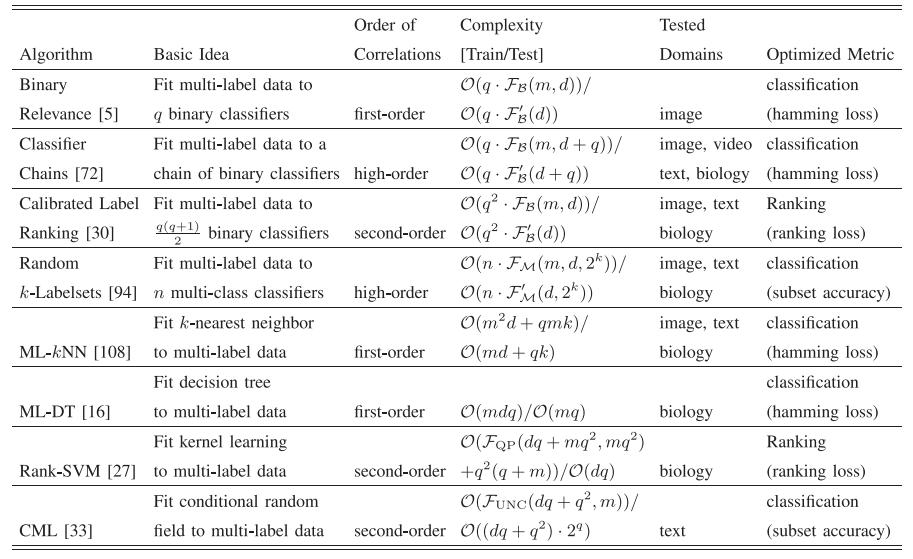
\includegraphics[scale = 0.45]{images/summary.png}
\caption{Summary of Representative Multi-Label Learning Algorithms}
\end{center}
\end{figure}
\end{frame}
%------------------------------------------------
\section{Related Learning Methods}
%------------------------------------------------
\begin{frame}
\frametitle{\insertsection}
\begin{itemize}
\item[$\bullet$] <2-> Multi-instance learning
\begin{itemize}
\item[$\circ$] <3-> Instead of labeled instances, get binary-labeled \emph{bags of instances}
\item[$\circ$] <4-> Assign positive label to bag if at least one member is positive
\item[$\circ$] <5-> Models complex semantics of $x_i$ in input space, rather than its output
\end{itemize}
\item[$\bullet$] <6-> Ordinal classification
\begin{itemize}
\item[$\circ$] <7-> Assume label relevance is not binary, but soft
\item[$\circ$] <8-> Produce a vector of ordinal graded membership
\item[$\circ$] <9-> Transform M-L problem to a set of ordinal set of problems
\end{itemize}
\item[$\bullet$] <10-> Multi-task learning
\begin{itemize}
\item[$\circ$] <11-> Multiple tasks trained in parallel, sharing information
\item[$\circ$] <12-> Knowledge from related tasks used as an inductive bias to improve generalization
\item[$\circ$] <13-> Shared or different feature space, small task workload
\end{itemize}
\item[$\bullet$] <14-> Data streams classification
\begin{itemize}
\item[$\circ$] <15-> Real-world objects are generated online and processed in  real-time
\item[$\circ$] <16-> Concept drift problem
\end{itemize}
\end{itemize}
\end{frame}

%------------------------------------------------
\section{Conclusion}
%------------------------------------------------
\begin{frame}
\Huge{\centerline{Conclusion}}
\end{frame}
%------------------------------------------------
\begin{frame}
\frametitle{\insertsection}
\onslide <2->{Summary:}
\begin{itemize}
\item[$\bullet$] <3-> Multi-label learning problem definition
\item[$\bullet$] <4-> Multi-label learning representative algorithms
\item[$\bullet$] <5-> Related learning methods
\end{itemize}

\onslide <6->{Future goals:}
\begin{itemize}
\item[$\bullet$] <7-> Formal characterization on the underlying concept / mechanism on the appropriate usage of label correlations, especially on large output spaces
\item[$\bullet$] <8-> Thorough experimental comparative study to discover pros and cons of different multi-label learning algorithms
\end{itemize}
\end{frame}

%------------------------------------------------
\subsection{Online resources}
\begin{frame}
\frametitle{\insertsection : \insertsubsection}
\begin{figure}
	\begin{center}
		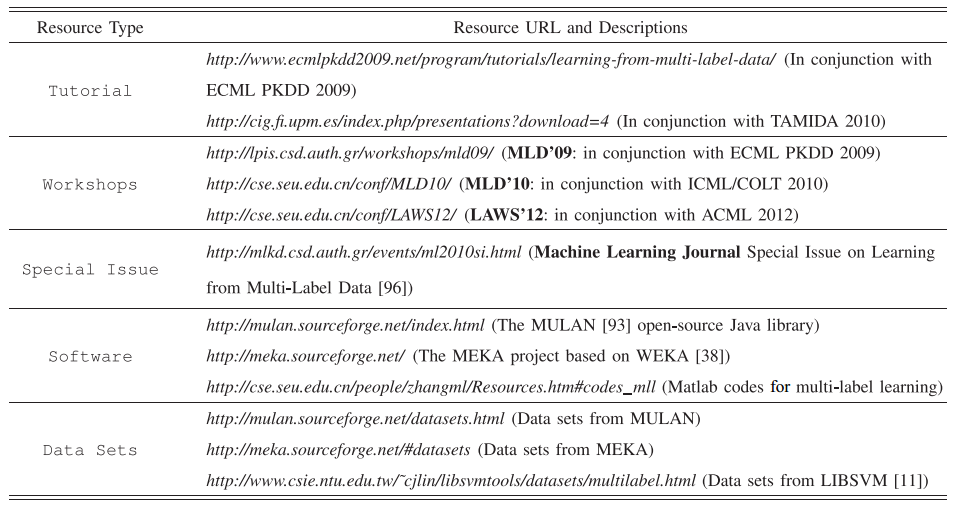
\includegraphics[scale = 0.47]{images/online.png}
		\caption{Online Resources for Multi-Label Learning}
	\end{center}
\end{figure}
\end{frame}
%------------------------------------------------
\subsection{Related Work}
\begin{frame}
\frametitle{\insertsection : \insertsubsection}
\begin{itemize}
\item[$\bullet$] Madjarov, Gjorgji, et al. "An extensive experimental comparison of methods for multi-label learning." Pattern Recognition 45.9 (2012): 3084-3104
\item[$\bullet$] Tsoumakas, Grigorios, and Ioannis Katakis. "Multi-label classification: An overview." International Journal of Data Warehousing and Mining 3.3 (2006)
\item[$\bullet$] Zhang, Min-Ling, and Kun Zhang. "Multi-label learning by exploiting label dependency." Proceedings of the 16th ACM SIGKDD international conference on Knowledge discovery and data mining. ACM, 2010
\end{itemize}
\end{frame}
%------------------------------------------------

\subsection{Additional Bibliography}
\begin{frame}
\frametitle{\insertsection : \insertsubsection}
\begin{itemize}
\item[$\bullet$] Vens, Celine, et al. "Decision trees for hierarchical multi-label classification." Machine Learning 73.2 (2008): 185-214.
\item[$\bullet$] Tsoumakas, Grigorios, and Ioannis Vlahavas. "Random k-labelsets: An ensemble method for multilabel classification." Machine learning: ECML 2007 (2007): 406-417.
\item[$\bullet$] Zhang, Min-Ling, and Zhi-Hua Zhou. "ML-KNN: A lazy learning approach to multi-label learning." Pattern recognition 40.7 (2007): 2038-2048.
\item[$\bullet$] Elisseeff, André, and Jason Weston. "A kernel method for multi-labelled classification." Advances in neural information processing systems. 2002.
\item[$\bullet$]  Ghamrawi, Nadia, and Andrew McCallum. "Collective multi-label classification." Proceedings of the 14th ACM international conference on Information and knowledge management. ACM, 2005.
\item[$\bullet$]  Cheng, Weiwei, Eyke Hüllermeier, and Krzysztof J. Dembczynski. "Graded multilabel classification: The ordinal case." Proceedings of the 27th international conference on machine learning (ICML-10). 2010.
\end{itemize}
\end{frame}
%------------------------------------------------
\section{The end}
\begin{frame}
\Huge{\centerline{Thank you}}
\Huge{\centerline{Questions?}}
\end{frame}
%------------------------------------------------
\end{document}
